%__INSERT_LICENSE__
\Section{Gatherers and embedded gatherers}

Typically \emph{``gatherers''} are reduction operators over the
element sets, i.e. instead of assembling a matrix or vector, the
gather operations produce some kind of global data, as for instance
%
\begin{itemize}
\compactlist 
\item The volume/surface/length of an elemset.
\item The integral of some quantity (fields, coordinates, or functions
  of the them) over the element set, for instance total concentration,
  total energy, total (linear or angular) momentum or angular
  momentum. 
\item Same as above but depending also on gradients of the state
  variables, for instance: total elastic energy. This involves some 
\item Same as above but integrals of quantities on a manifold of a
  dimension lower than the embedding space. In this case the integrand
  may involve also the normal to the surface, for instance total flow
  of heat or volume rate through a surface. 
\end{itemize}
 
Gatherers are implemented as \verb+elemsets+ the only difference is
that they typically only process a special jobinfo named
\verb+gather+. This jobinfo is processed after the time step,
i.e. only after the Newton loop, on the converged values. This jobinfo
task does not assemble vectors or matrices, but a series global values
stored in a global C++ vector called
\verb+vector<int> gather_values+. A typical call is as follows (taken
from \verb+ns.cpp+),
%
\medskip
\begin{verbatim}
    arglf.clear();
    arglf.arg_add(&state,IN_VECTOR|USE_TIME_DATA);
    arglf.arg_add(&state_old,IN_VECTOR|USE_TIME_DATA);
    arglf.arg_add(&gather_values,VECTOR_ADD);
    ierr = assemble(mesh,arglf,dofmap,"gather",&time_star);
    CHKERRA(ierr);
\end{verbatim}
\medskip
%
Note that three arguments are passed to the \verb+gather+ assemble
task: the old and new states, and the vector of gathered values. 

Many gatherer elemsets have the suffix \verb+integrator+ appended to
their names, for instance \verb+visc_force_integrator+ or
\verb+volume_integrator+

%<*>---<*>---<*>---<*>---<*>---<*>---<*>---<*>---<*>---<*>---<*>
\subsection{Dimensioning the values vector} 

In order to use the gatherers the user must before dimension
appropriately the array of values with global option
\verb+ngather+. Then, for each gatherer elemset the user must set the
options that select a continuous range in this vector, namely
\verb+gather_pos+ and \verb+gather_length+. The selected range is
\verb|[gather_pos,gather_pos+gather_length]|. Then, for instance, if
the (hyopthetical) gatherer elemset \verb+momentum_integrator+ is
supposed to compute the integral of the momentum (a 3-vector in 3D),
then we could use as

\medskip
\begin{verbatim}
global_options
...
ngather 3
__END_HASH__

elemset momentum_integrator 4
...
gather_pos 0
gather_length 3
data ./connectivity.dat
__END_HASH
\end{verbatim}
\medskip
%
With this setup, the program will compute for each time step the
integral of the momentum, at will print these three values on stadard
output. If a string is passed to the global option \verb+gather_file+
for instance
%
\medskip
\begin{verbatim}
...
ngather 3
gather_file momentum.out
...
\end{verbatim}
\medskip
%
then, instead of reporting the gathered values on standard output they
are printed on the corresponding file. The file is opened and closed
at each time step. 

%<*>---<*>---<*>---<*>---<*>---<*>---<*>---<*>---<*>---<*>---<*>
\subsection{Embedded gatherers} 

%<*>---<*>---<*>---<*>---<*>---<*>---<*>---<*>---<*>---<*>---<*> 
\begin{figure*}[htb]
\centerline{\includegraphics{./OBJ/embgath}}
\caption{Embedded gatherer element}
\label{fg:embgath}
\end{figure*}
%<*>---<*>---<*>---<*>---<*>---<*>---<*>---<*>---<*>---<*>---<*> 

If the elemset has a dimension lower than the embedding space, for
instance a surface embedded in 3D space, then computing the gradients
of the variables on the surface can not be done with the information
on the surface only. This is not an uncommon situation, for instance
it happens when computing viscous forces of a Newtonian fluid on the
skin of a solid body. The \emph{gradient} of the velocity field must
be computed in order to compute the stress on the skin. But 
if the velocity field is known only on the surface (think, for
simplicity, in the case a of plane surface) the normal component of
the gradient can not be determined. 

In order to solve this, a special class of gatherers have been
developed, namely the \verb+embedded_gatherer+ class. Tipically such
an elemset is composed is a surface elemset, associated with a volume
one. For instance (see figure~\ref{fg:embgath}) the user can have a
fluid problem with a volume elemset (in 2D) composed of
\verb+cartesian2d+ and wants to compute the viscous traction on the
solid surface $AB$. For this, she adds an elemset
\verb+visc_force_integrator+ composed of six-nodes elements composed
of three layers of segments parallel to the surface as, for instance,
the element 3-4-8-9-14 (marked with a dashed line in the figure). 
This special elements can be seen as layers of surface elements,
parallel to the skin. With the velocity values computed by the
Navier-Stokes solver at these nodes, the gatherer elemset can compute
high precision approximations to the normal derivatives of velocity at
the surface. 

\begin{itemize}
\compactlist 

\item Note that this requires that the mesh must be somewhat
  structured near the surface. However, it is usual to add structured
  layer on the body skin in order to correctly capture the boundary
  layer.

\item Also, it requires the construction of the connnectivities of
  these layers, what may be cumbersome, but we will see later that
  this can be done automatically (see \S\ref{sec:auto-emb}).  

\item The size of the elements in the normal direction are not
  required to be equispaced, i.e. the distances 1-6 and 6-11 are not
  required to be equal or similar. This is important, because normally
  the layers of nodes are refined towards the surface, as shown in the
  figure. 

\item The lines of nodes are not required to be normal to the
  surface. 

\item However, it is required that each row of nodes (for instance the
  row 1-6-10) must \emph{lay on a smooth curve}. This is required,
  since in the process of computing high normal derivatives a Taylor
  expansion is computed in terms of this curves, so the error depends
  on the higher derivatives (e.g. the curvature) of the line. 

\end{itemize}

The typical invocation is as follows
%
\medskip
\begin{verbatim}
elemset nsi_tet_les_full 4
geometry cartesian2d
__END_HASH__
1 2 7 6
6 7 12 11
2 3 8 7
...
__END__ELEMSET__

elemset visc_force_integrator 6
geometry line2quad
__END_HASH__
1 2 6 7 11 12
2 3 7 8 12 13
3 4 8 9 13 14
...
__END__ELEMSET__
\end{verbatim}
\medskip

%<*>---<*>---<*>---<*>---<*>---<*>---<*>---<*>---<*>---<*>---<*> 
\begin{figure*}[htb]
\centerline{\includegraphics{./OBJ/embgath2}}
\caption{Embedded gatherer elements in 3D}
\label{fg:embgath2}
\end{figure*}
%<*>---<*>---<*>---<*>---<*>---<*>---<*>---<*>---<*>---<*>---<*> 

Note that the geometry is special \verb+line2quad+ means that the
surface geomtry are lines and the corresponding volume elemset is
composed of quads. The other two possibilities implemented so far are
\verb+tri2prism+ and \verb+quad2hexa+ (see figure~\ref{fg:embgath2}).

Typical invocation is as follows
The typical invocation is as follows
%
\medskip
\begin{verbatim}
elemset visc_force_integrator 9
geometry tri2prism
__END_HASH__
...
1 2 3 4 5 6 7 8 9
...
__END__ELEMSET__
\end{verbatim}
\medskip
%
and
%
\medskip
\begin{verbatim}
elemset visc_force_integrator 12
geometry quad2hexa
__END_HASH__
...
1 2 3 4 5 6 7 8 9 10 11 12
...
__END__ELEMSET__
\end{verbatim}
\medskip

%<*>---<*>---<*>---<*>---<*>---<*>---<*>---<*>---<*>---<*>---<*>
\subsection{Automatic computation of layer connectivities} 
\label{sec:auto-emb}  

Sometimes it is somewhat cumbersome to compute the connectivities of
the embedded gatherer connectivities since it involves the finding of
layers of nodes inside the adjacent volume element. This can be done
automatically by PETSc-FEM if the \verb+identify_volume_elements+ is
activated and the name of the adjacent volume element is passed
through the option \verb+volume_elemset+ for instance
%
\medskip
\begin{verbatim}
elemset nsi_tet_les_full 4
geometry cartesian2d
name viscous_fluid
__END_HASH__
1 2 7 6
6 7 12 11
2 3 8 7
...
__END__ELEMSET__

elemset visc_force_integrator 6
volume_elemset viscous_fluid
identify_volume_elements
geometry line2quad
__END_HASH__
1 2 1 1 1 1
2 3 1 1 1 1
3 4 1 1 1 1
...
__END__ELEMSET__
\end{verbatim}
\medskip
%
Note that the nodes in the inner layers of nodes are replaced by 1's. 
With this setting, the code will inspect the connectivity of the
\verb+viscous_fluid+ elemset and find the nodes corresponding to the
inner layers and replace the 1's by the correct n ode number. 

%<*>---<*>---<*>---<*>---<*>---<*>---<*>---<*>---<*>---<*>---<*>
\subsection{Passing element contributions as per-element properties} 

For some applications it is desirable to have the individual element
contributions instead of having their sum. For instance, in a
fluid-structure application involving a fluid and a deformable solid,
it does not suffice only with the integral of the forces to compute
the evolution of the solid, but also it is needed the whole
distribution of forces. In this case what is needed is a list of
surface elements and the total force for each element. 

This behavior can be activated with the \verb+pass_values_as_gather+
option. This mechanism can be activated \emph{in addition} to the usual
global \verb+gather_values+ mechanism. The global vector mechanism can
be deactivated by setting the \verb+gather_length+ to 0, or not
setting it at all. In summary
%
\begin{itemize}
\compactlist 
\item If \verb+gather_length>0+  and 
  \verb+pass_values_as_gather==0+ only the usual 
  \verb+gather_values+ mechanism is activated.
\item If \verb+gather_length>0+  and 
  \verb+pass_values_as_gather==1+ both mechanisms 
  are activated. 
\item If \verb+gather_length==0+ and 
  \verb+pass_values_as_gather==1+
  only the per-element mechanism is activated. The amount of values to
  be computed is set with the \verb+store_values_length+ option. 
\end{itemize}
%
The summary of relevant options is
%
\begin{itemize}
\compactlist 
\item \verb+pass_values_as_gather+ activates the mechanism of passing per
  element computed values as per-element properties. 

\item \verb+store_values_length+ is an integer indicating how many values
  are computed by the gatherer. It defaults to
  \verb+gather_length+. However, if the standard mechanism of the
  \verb+gather_values+ is deactivated, then the number of computed
  values must be passed through this option. 

\item \verb+store_in_property_name+ is a string that identifies the
  per-element property that must be filled with the computed values. 
  Of course, the user must define such property with the appropriate
  size. The values in the connectivity table are irrelevant (for
  instance null values) and will be overwritten by the gatherer. 
\end{itemize}

%<*>---<*>---<*>---<*>---<*>---<*>---<*>---<*>---<*>---<*>---<*>
\subsection{Parallel aspects} 

Of course, PETSc-FEM is in charge of adding the contributions on
different processors. The resulting sum of contributions over
\emph{all elements} in \emph{all procesors}.  The sum is available not
only in the master (\verb+rank=0+), but in all processors (as with an
\verb+MPI_Allreduce()+ call).  This is important since this global sum
can be used also in \emph{hooks} in order to perform computations.
For instance, a gatherer can be used to compute the force on a body,
and this force can be passed to a hook to compute the movement of the
body.

%<*>---<*>---<*>---<*>---<*>---<*>---<*>---<*>---<*>---<*>---<*>
\subsection{Creating a gatherer} 

Typically a gatherer is created by deriving from the virtual class
\verb+gatherer+ and implementing the \verb+set_pg_values()+ method
which is in charge of computing the integrands.
%
\medskip
\begin{verbatim}
class gatherer {
// ...
public:
  // perform several checks and initialization
  void init();
  // add Gauss point contributions
  void set_pg_values(vector<double> &pg_values,FastMat2 &u,
		     FastMat2 &uold,FastMat2 &xpg,FastMat2 &Jaco,
		     double wpgdet,double time);
};
\end{verbatim}
\medskip
%
\begin{itemize}
\compactlist 
\item The \verb+init()+ function may be used for initialization. The
  \verb+TGETOPTDEF(thash,....)+ macro can be used for extracting
  options of the elemset. For instance,
%
\medskip
\begin{verbatim}
TGETOPTDEF(thash,double,Young_modulus,0.);
\end{verbatim}
\medskip 

\item The \verb+set_pg_values(...)+ is the main method. Here the user
  computes the values to be integrated. Its signature is
%
\medskip
\begin{verbatim}
  virtual void set_pg_values(vector<double> &pg_values,FastMat2 &u,
		     FastMat2 &uold,FastMat2 &xpg,FastMat2 &n,
		     double wpgdet,double time)=0;
\end{verbatim}
\medskip
%
The argument \verb+pg_values+ are the values to be computed. (\verb+pg+
stands for Gauss point, since usually this function is called by the
gatherer class at the Gauss points of integration.) \verb+u+ and
\verb+uold+  are the states at times $t^n$ and $t^{n+1}$. \verb+xpg+
are the coordinates of the Gauss point. \verb+n+ is the normal to the
surface (only relevant if the dimension of the element \verb+ndimel+
is equal to \verb+ndim-1+). \verb+wpgdet+ is the area of the Gauss
point (i.e. the Gauss point weight times the Jacobian of the
transformation to the master element). 

\item Other methods are \verb+void element_hook(int k)+ which is
  called \emph{before} the Gauss point hook and then can be used in
  order to pre-compute some stuff for all the Gauss points. \verb+k+
  is the element number. Finally \verb+void clean()+ can be used after
  processing all the elements and doing some cleanup. 

\end{itemize}

% Local Variables: *
% mode: latex *
% tex-main-file: "petscfem.tex" *
% End: *

